\usepackage{amsmath}

Los \textit{Mel Frequency Cepstral Coefficients} (MFCC)~\cite{Davis80} son coeficientes para la representación del habla basados en la percepción auditiva humana.
Su objetivo es caracterizar el contenido relevante de la señal, obviando aquellas características que poseen información poco valiosa como el ruido de fondo, emociones, volumen, tono, etc.
Si bien fueron desarrollados para tareas asociadas al reconocimiento automático del habla, igualmente han tenido una amplia aplicación en áreas relacionadas al procesamiento de señales musicales y bioacústicas~\cite{Clemins05,Cowling03,Dufour14,Fagerlund07,Lee06,Li01,McKinney03,Mitrovic06}.

Los MFCC se basan en la característica del sistema auditivo humano que provoca que para este sea más difícil discernir entre dos frecuencias cercanas cuanto más altas ellas sean.
La \textbf{escala Mel} (figura~\ref{img:mel-scale}) fue desarrollada con el propósito de representar dicha propiedad, permitiendo medir las frecuencias de un modo más acorde a la percepción humana de estas, mediante el uso de la unidad de medida conocida como \textit{mel}.

\begin{figure}[!h]
    \centering
    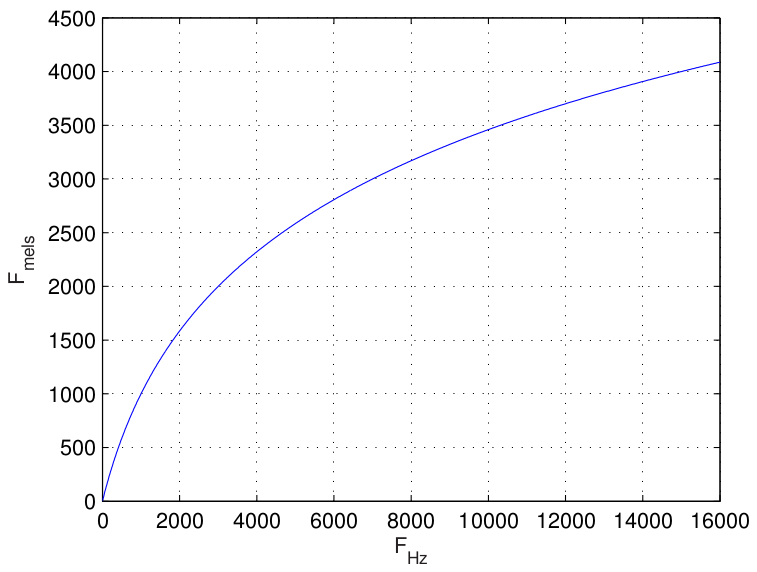
\includegraphics[width=0.5\textwidth]{mel-scale.png}
    \caption{Correspondencia entre las unidades de medida de frecuencias \textit{hertz} y \textit{mel} de acuerdo con la escala Mel.}
    \label{img:mel-scale}
\end{figure}

La conversión de hertz ($f$) a mel ($m$) se realiza aplicando la ecuación~(\ref{eq:Hz-Mel}), mientras que por~(\ref{eq:Mel-Hz}) se puede convertir en sentido contrario.

\begin{gather}
    \label{eq:Hz-Mel}
    m = 2595\log_{10}\left( 1 + \frac{f}{700} \right)

    \label{eq:Mel-Hz}
    f = 700\left( 10^{m/2595} - 1 \right)
\end{gather}

Una ventaja de la escala Mel es que nos permite definir los llamados \textbf{bancos de filtros de Mel}, mediante los cuales se <<resume>> la energía de una señal en $M$ bandas repartidas en correspondencia con la escala Mel (más distanciadas a medida que las frecuencias se hacen mayores).
Para ello, se divide el intervalo de frecuencias presente en la señal en $M+2$ puntos igualmente distanciados.
A continuación se convierten a Mel, de forma que ahora estos estarán situados a distancias correspondientes a la percepción humana de las frecuencias.
Luego, los $M$ filtros son definidos mediante la siguiente fórmula:

\begin{equation}
    \label{eq:Mel filterbank}
    H_m(k) = \begin{cases}
                 0 & k < f_{m-1} \\
                 \frac{k-f_{m-1}}{f_m - f_{m-1}} & f_{m-1}\leq k\leq f_m \\
                 \frac{f_{m+1}-k}{f_{m+1}-f_m} & f_m \leq k\leq f_{m+1} \\
                 0 & k > f_{m+1} \\
    \end{cases}
\end{equation}

\noindent
donde $f_m$ es la frecuencia correspondiente al $m$-ésimo punto del intervalo.
La representación gráfica de un resultado de la aplicación del procedimiento anterior puede observarse en la figura~\ref{img:mel-filters}.

\begin{figure}[!h]
    \centering
    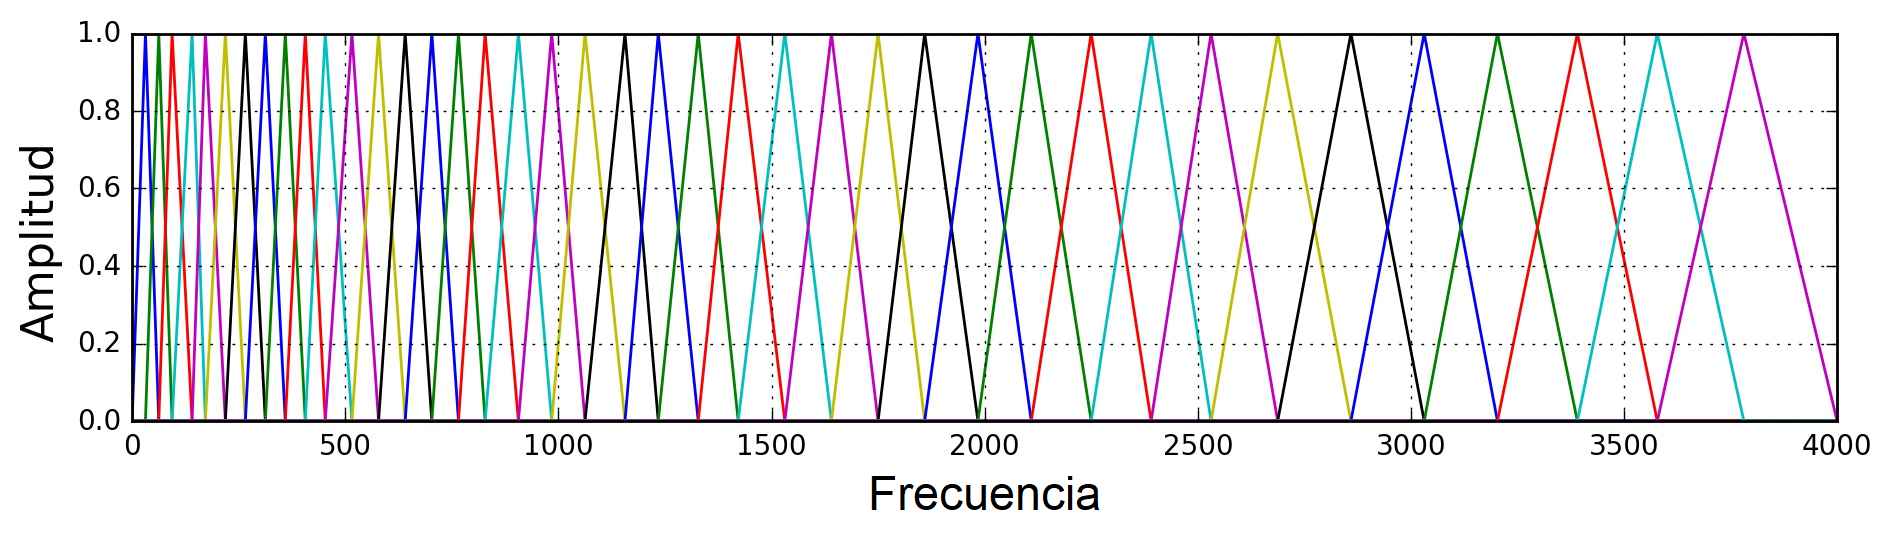
\includegraphics[width=\textwidth]{mel-filters.png}
    \caption{Banco de 40 filtros de Mel en el intervalo de frecuencias de 0~Hz a 4~000~Hz.}
    \label{img:mel-filters}
\end{figure}

A partir de todo lo anterior puede plantearse el algoritmo para el cálculo de los MFCC como sigue:

\begin{algorithm}
    \caption{Cálculo de los MFCC}
    \label{algorithm:MFCC}
    Descomponer la señal $s[n]$ en tramas $s[n]_m = x[n]$ aplicando una función ventana\;
    Por cada trama calcular la potencia espectral (periodograma) a partir de su DFT, cuya $k$-ésima componente se calcula mediante la ecuación
    \begin{equation*}
        P[k] = \frac{|X[k]|^2}{K}
    \end{equation*}
    donde $K$ es la dimensión de la DFT de la trama\;
    Aplicar el banco de filtros de Mel a $P[k]$ y sumar las energías de cada filtro.
    Aplicando $M$ filtros, se obtendrá entonces un vector de $M$ componentes (energías)\;
    Calcular el logaritmo de las energías\;
    Aplicar la transformada de coseno discreta (DCT) al vector de los logaritmos\;
\end{algorithm}

Los pasos del 1 al 4 cumplen la meta de lograr un <<resumen>> de la energía presente en la señal que se corresponda con la percepción humana del sonido.
El paso número 5, persigue eliminar la correlación entre los coeficientes.
Gracias a la aplicación de la DCT, se obtiene un vector de componentes independientes entre sí (no correlacionadas), y por lo tanto este puede ser utilizado en otros procedimientos que así lo requieran.

La DCT se calcula mediante la siguiente ecuación:
\begin{equation}
    \label{eq:DCT}
    f[j] = \sum_{m=0}^{M-1}{e[m]\cos{\left[ \frac{\pi}{M}j\left( m + \frac{1}{2} \right) \right]}}
\end{equation}

Generalmente se usan bancos de entre 20 y 40 filtros y solamente se conservan los primeros 12 o 13 coeficientes;
esto último debido a que la representación obtenida a partir de la aplicación de la DCT suele comprimir la información relevante en los primeros coeficientes, quedando poco valor en los más altos~\cite{Davis80}.

\begin{figure}[!h]
    \centering
    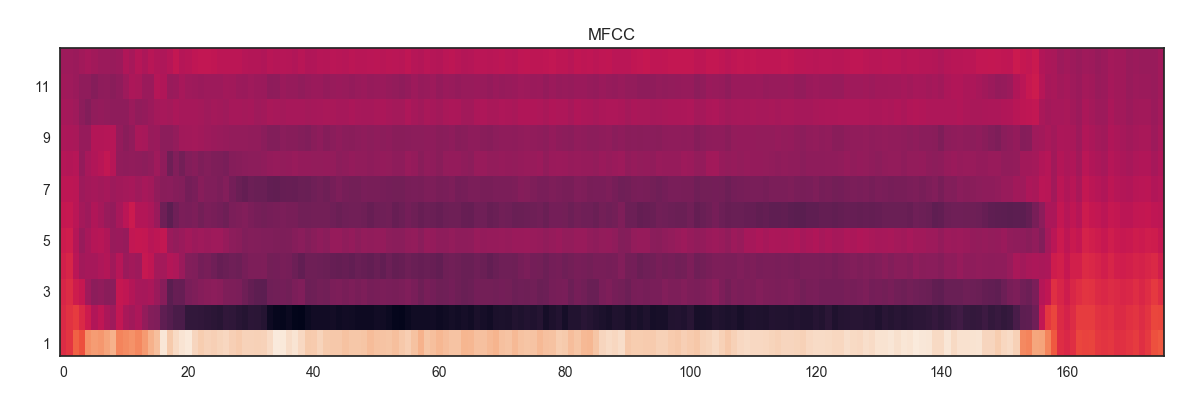
\includegraphics[width=\textwidth]{mfcc.png}
    \caption{MFCC (coeficientes del 1 al 12) del sonido de la figura~\ref{img:oscillogram}.}
    \label{img:mfcc}
\end{figure}

Los coeficientes \textbf{delta} y \textbf{delta-delta}, también conocidos como \textit{diferenciales} y \textit{de aceleración} respectivamente,
constituyen una posible mejora al vector de los MFCC\@.
Estos incluyen información relativa al comportamiento de la energía espectral en el tiempo, que complementa la información estática de una trama que recogen los MFCC\@.
Para calcular los coeficientes delta se aplica la siguiente fórmula:

\begin{equation}
    \label{eq:delta}
    d_t = \frac{\sum_{n=1}^{T}{n(c_{t+n} - c_{t-n})}}{2\sum_{n=1}^{T}{n^2}}
\end{equation}

\noindent
donde $d_t$ es el vector de coeficientes delta correspondiente a la trama $t$, y $c_{t+n}$ y $c_{t-n}$ son los MFCC de las tramas posteriores y anteriores respectivamente.
El valor de la cantidad de tramas consecutivas a explorar ($T$) suele ser 2.

Los coeficientes delta-delta pueden ser calculados de igual forma aplicando~(\ref{eq:delta}) empleando los delta en lugar de los MFCC\@.

A menudo sucede que un segmento de audio está compuesto por más de una trama, de manera que los procedimientos que se han descrito en esta sección producen no un único vector de características sino uno por cada trama del segmento.
Una posible solución a esta situación consiste en construir un único vector, con los promedios componente a componente de todos los de la secuencia obtenida~\cite{Fagerlund07,Lee06}.